\section{Details of Performance Test Conclusions}
\label{appendix:planning}

In the course of our performance comparisons, we were able to characterize some scenarios in which the two systems displayed definably different behavior.
In this appendix, we define those scenarios, and we discuss some possible causes for those differences.
However, before doing either of those things, it is necessary to explain the set of experiments which provide the explanitory framework for this section.

\subsection{Query Planning}

In this section, we discuss differences in performance that we noticed in experiments on the GDELT dataset, which is composed of points.
At an abstract level, the point-storage mechanisms found in the respective systems are esentially equally capable.
(GeoMesa uses a Z-index and GeoWave uses a more sophisticated Hilbert-index, but that difference should not generate much of performance discrepency in-and-of itself.)
Since we did observe some systematic differences in performance, we must look beyond the modest high-level differences to try to find an answer.

Query-planning, the process of converting a query from the user into a collection of row-ranges to be submitted to Accumulo, is the highest-level significant algorithmic difference between the two systems that we have been able to identify (at least for point queries).
GeoWave uses a sophisticated uzaygezen (\url{https://github.com/aioaneid/uzaygezen}) library to compute its query plans,
and GeoMesa uses a faster (but less thorough) sfcurve (\url{https://github.com/locationtech/sfcurve}) library.
The net effect is that GeoWave tends to spend more time on query planning,
but with greater selectivity (fewer false-positives in the ranges which must later be filtered out).

\subsection{Query Planning Experiments}

We performed a series of query planning experiments which mirror our GDELT experiments.
In an earlier section, we described a set of experiments in which we performed buffered queries around city centers using the GDELT dataset; here we used the excact same set \texttt{CQL} queries that were generated in the experimenet, but we gather different data.
That was done by isolating the parts of the respective systems responsible for query-planning and putting them into stand-alone programs (\url{https://github.com/azavea/geowave-geomesa-comparative-analysis/tree/master/query-planning}).

We used those stand-alone programs to measure the amount of time spent on query-planning, as well as the results of the planning (the number of ranges generated and the lengths of those ranges).

\subsubsection{By Diameter}

Allowing the diameter of the buffer around each city center to scale from $10$ kilometers to $650$ kilometers,
we obtained the results shown in Figure \ref{planningsizetime}.

\begin{figure}[h!tb]
  \centering
  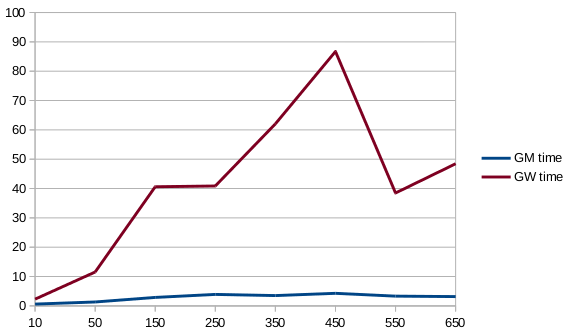
\includegraphics[width=0.40\textwidth]{../docs/img/query-planning/size-time.png}
  \caption{Query planning: time versus query size.}
  \label{planningsizetime}
\end{figure}

The graphs in that figure shows the average amount of time (in milliseconds) that each system spent in the query-planning phase for all queries of the given diameter.
Here we observe that GeoWave takes much longer to complete this phase (although it should be noted that these experiments were performed on a differently-configured computer than GDELT experiment was, so the timings are not directly comparable).

\begin{figure}[h!tb]
  \centering
  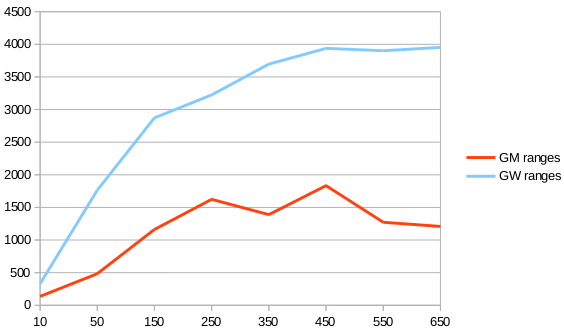
\includegraphics[width=0.40\textwidth]{../docs/img/query-planning/size-ranges.png}
  \caption{Query planning: ranges versus query size.}
  \label{planningsizeranges}
\end{figure}

The graph in Figure \ref{planningsizeranges} shows the number of ranges generated by the two systems.
We see that GeoWave generates many more ranges over the range of diameters.

\begin{figure}[h!tb]
  \centering
  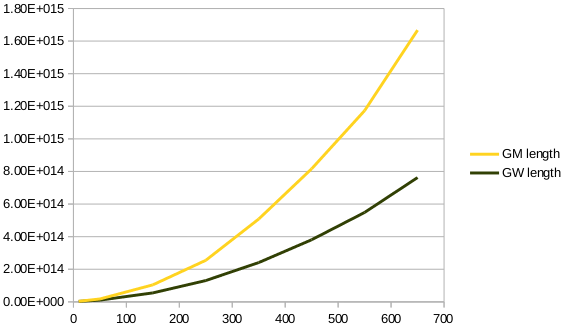
\includegraphics[width=0.40\textwidth]{../docs/img/query-planning/size-length.png}
  \caption{Query planning: total length of ranges versus query size.}
  \label{planningsizelength}
\end{figure}

The graph in Figure \ref{planningsizelength} shows the total length of the ranges (difference between the respective starting and ending indices of the ranges) generated by the two systems.
Here we see that GeoMesa's total is much greater, as much as a factor of ten for larger query windows.
This particular number becomes relatively more important in areas of greater data density.
Taken together with the number of ranges (displayed in Figure \ref{planningsizeranges}), this quantity gives us an idea of the selectivity of the query planner.

\subsubsection{By Time Window}

The same data can also be broken-down according to the temporal width of the queries.

\begin{figure}[h!tb]
  \centering
  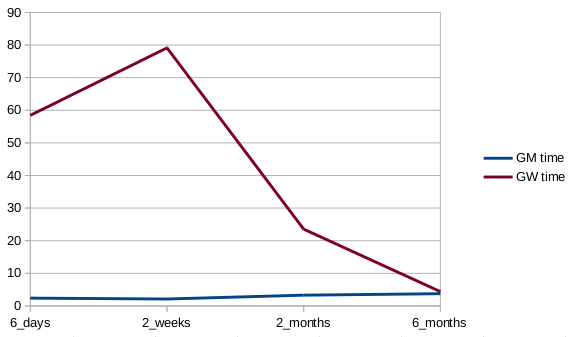
\includegraphics[width=0.40\textwidth]{../docs/img/query-planning/window-times.png}
  \caption{Query planning: time versus temporal width.}
  \label{planningtimetime}
\end{figure}

The graph in Figure \ref{planningtimetime} shows the query-planning time required by the two systems as a function of the temporal width of the queries.
Although the GeoMesa query-planning time is generally greater than that of GeoMesa, in this particular case we see that the two actually coincide at the ``$6$ month'' mark.
That fact will be important to us later.

\begin{figure}[h!tb]
  \centering
  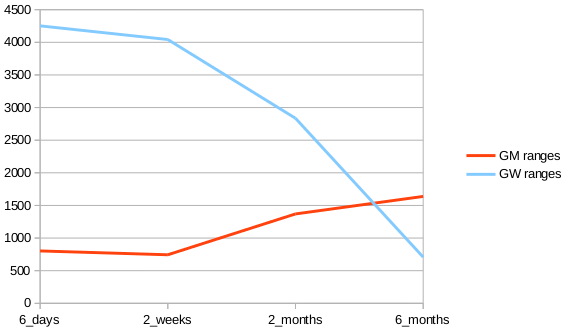
\includegraphics[width=0.40\textwidth]{../docs/img/query-planning/window-ranges.png}
  \caption{Query planning: ranges versus temporal width.}
  \label{planningtimeranges}
\end{figure}

The graph in Figure \ref{planningtimeranges} shows the number of ranges generated as a function of temporal widths.
Although GeoMesa normally has a larger number, in this case we see GeoMesa actually produce fewer ranges than GeoMesa at ``$6$ month''.
This is mildly surprising (based on a number of other experiments that we have performed) and will once again be important later.

\begin{figure}[h!tb]
  \centering
  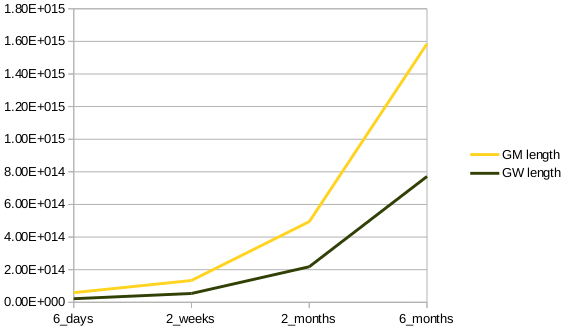
\includegraphics[width=0.40\textwidth]{../docs/img/query-planning/window-length.png}
  \caption{Query planning: total range length versus temporal width.}
  \label{planningtimelength}
\end{figure}

Finally, the graph in Figure \ref{planningtimelength} shows the aggregate query-plan length as a function of temporal window width.
As before, GeoWave remains consistently lower in this area.

\subsection{Performance Observations vis-a-vis Query Planning}

In those experiments, GeoMesa tended to do better than GeoWave as the size of the result sets increased.
Conversely, we also found that GeoWave performs better as the selectively of the query increases.
Examination of the respective query-planning strategies of the systems shows that GeoMesa submits fewer ranges of keys to Accumulo, but those ranges are wider in length.
These fewer-but-larger ranges could provide an advantage in this context.

Although GeoMesa tends to do better than GeoWave on the queries just described, GeoMesa's relative performance advantage lessens as the temporal widths of the queries increases.
GeoWave tends to produce sets of ranges whose counts goes down as the temporal window widens, whereas GeoMesa produces sets of increasing size.
Simultaneously, the sum of the widths of GeoWave's intervals are smaller than those of GeoWave.

Another pattern that we noticed is that GeoWave tends to do better on heavy load than GeoMesa on the GDELT dataset.
Once again looking to query-planning for an explination, the more-but-shorter ranges produced by GeoWave could provide an answer.
This creater selectivity could provide an advantage in which disk or network bandwidth is the limiting factor.
